% !TEX TS-program = pdflatex
% !TEX encoding = UTF-8 Unicode

% Matthew Urffer Master Thesis
% 
% Sim Performance
%
\section{Simulation Results}

%%%%%%%%%%%%%%%%%%%%%%%%%%%%%%%%%%%%%%%%%%%%%%%%%%%%%%%%%%%%%%%%%%%%%%%%%%%%%%%
%                                                                             %
%                                 Single Film                                 %
%                                                                             %
%%%%%%%%%%%%%%%%%%%%%%%%%%%%%%%%%%%%%%%%%%%%%%%%%%%%%%%%%%%%%%%%%%%%%%%%%%%%%%%
\subsection{Single Film}


%%%%%%%%%%%%%%%%%%%%%%%%%%%%%%%%%%%%%%%%%%%%%%%%%%%%%%%%%%%%%%%%%%%%%%%%%%%%%%%
%                                                                             %
%                                 Layered Films                               %
%                                                                             %
%%%%%%%%%%%%%%%%%%%%%%%%%%%%%%%%%%%%%%%%%%%%%%%%%%%%%%%%%%%%%%%%%%%%%%%%%%%%%%%
\subsection{Layered Films}
%%%%%%%%%%%%%%%%%%%%%%%%%%%%%%%%%%%%%%%%%%%%%%%%%%%%%%%%%%%%%%%%%%%%%%%%%%%%%%%
\begin{frame}{Effects of Layering I}
\small
\begin{itemize}
	\item Single films are unable to have a high enough count rate
	\item Solution: Multiple films!
	\item Effects of layering multiple films tested with EJ-426HD2
\end{itemize}
\begin{columns}[onlytextwidth]
\begin{column}{0.45\textwidth}
	\tiny
	\begin{figure}
		\centering
		\includegraphics[height=0.6\textheight]{images/EJ426HD_LayeredDetector_MultiSheet.eps}
	\end{figure}
\end{column}
\begin{column}{0.45\textwidth}
	\tiny
	\begin{figure}
		\centering
		\includegraphics[width=\textwidth]{images/EJ426HD_LayeredDetector_SingleSheet.eps}
	\end{figure}
\end{column}
\end{columns}
\end{frame}
%%%%%%%%%%%%%%%%%%%%%%%%%%%%%%%%%%%%%%%%%%%%%%%%%%%%%%%%%%%%%%%%%%%%%%%%%%%%%%%
\begin{frame}{Effects of Layering II}
Observe an increased neutron count rate \dots
	\begin{figure}
		\centering
		\includegraphics[height=0.6\textheight]{images/EJ426HD_Multi_NeutronComparison.eps}
		\small \caption{Neutron Spectra of EJ426HD2}
	\end{figure}
\end{frame}
%%%%%%%%%%%%%%%%%%%%%%%%%%%%%%%%%%%%%%%%%%%%%%%%%%%%%%%%%%%%%%%%%%%%%%%%%%%%%%%
\begin{frame}{Effects of Layering III}
with only a miminal increase in the gamma response!
\begin{columns}[onlytextwidth]
\begin{column}{0.45\textwidth}
	\tiny
	\begin{figure}
		\centering
		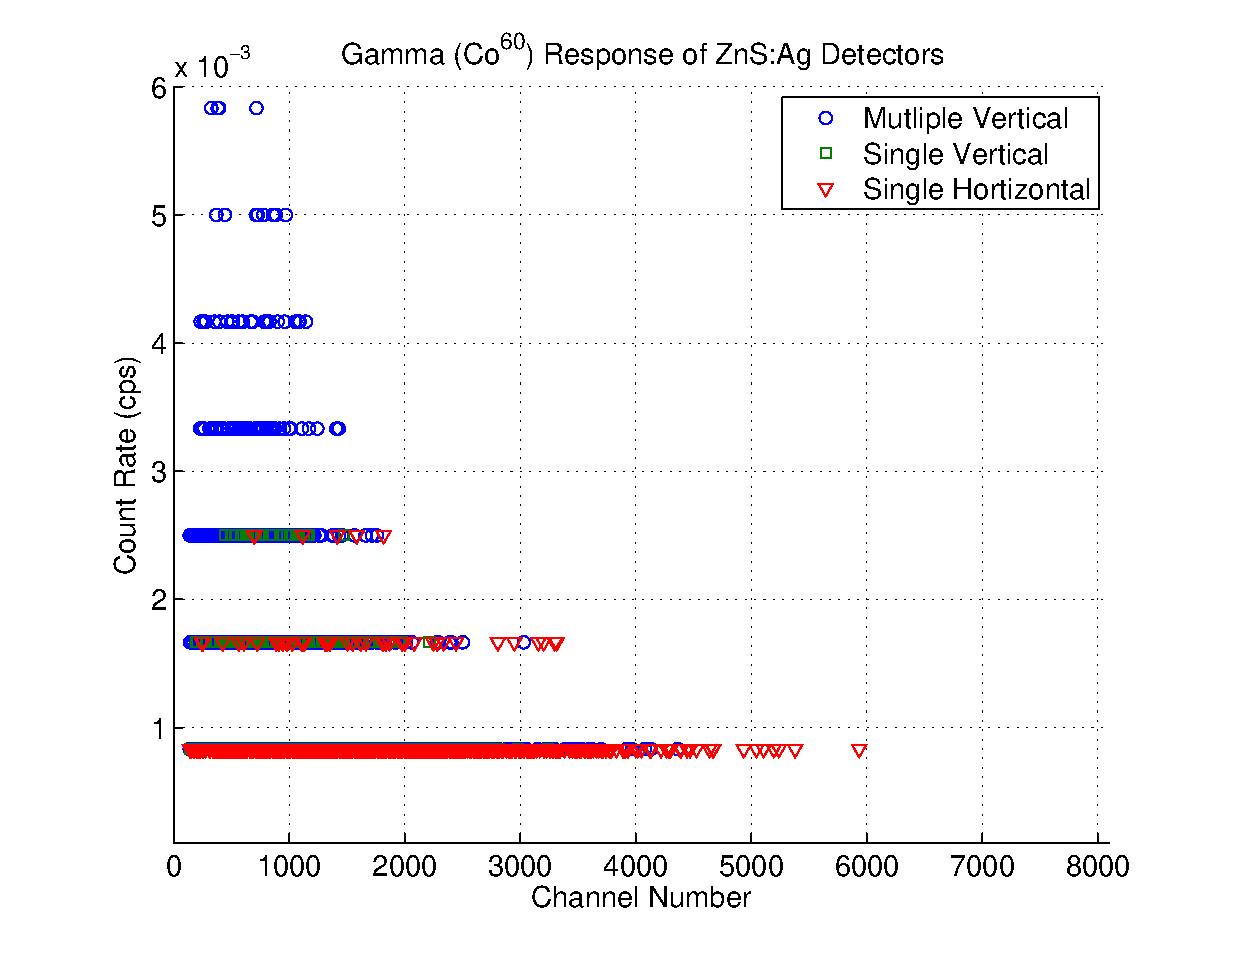
\includegraphics[width=\textwidth]{images/EJ426HD_Multi_GammaComparison.eps}
		\caption{Gamma Spectra of EJ426HD2}
	\end{figure}
\end{column}
\begin{column}{0.45\textwidth}
	\tiny
	\begin{figure}
		\centering
		\includegraphics[width=\textwidth]{images/EJ426HD_Multi_GammaIntEff.eps}
		\caption{Gamma Intrisinic Efficiency of EJ426-HD2}
\end{figure}
\end{column}
\end{columns}
\end{frame}
%%%%%%%%%%%%%%%%%%%%%%%%%%%%%%%%%%%%%%%%%%%%%%%%%%%%%%%%%%%%%%%%%%%%%%%%%%%%%%%
